%%%%%%%%%%%%%%%%%%%%%%%%%%%%%%%%%%%%%%%%%	
% a0poster Portrait Poster
% LaTeX Template
% Version 1.0 (22/06/13)
%
% The a0poster class was created by:
% Gerlinde Kettl and Matthias Weiser (tex@kettl.de)
% 
% This template has been downloaded from:
% http://www.LaTeXTemplates.com
%
% License:
% CC BY-NC-SA 3.0 (http://creativecommons.org/licenses/by-nc-sa/3.0/)
%
%%%%%%%%%%%%%%%%%%%%%%%%%%%%%%%%%%%%%%%%%

%----------------------------------------------------------------------------------------
%	PACKAGES AND OTHER DOCUMENT CONFIGURATIONS
%----------------------------------------------------------------------------------------

\documentclass[a0,portrait]{a0poster}

\usepackage{multicol} % This is so we can have multiple columns of text side-by-side
\columnsep=100pt % This is the amount of white space between the columns in the poster
\columnseprule=3pt % This is the thickness of the black line between the columns in the poster

\usepackage[svgnames]{xcolor} % Specify colors by their 'svgnames', for a full list of all colors available see here: http://www.latextemplates.com/svgnames-colors

\usepackage{times} % Use the times font
%\usepackage{palatino} % Uncomment to use the Palatino font

\usepackage{graphicx} % Required for including images
\graphicspath{{figures/}} % Location of the graphics files
\usepackage{booktabs} % Top and bottom rules for table
\usepackage[font=normalsize,labelfont=bf]{caption} % Required for specifying captions to tables and figures
\usepackage{amsfonts, amsmath, amsthm, amssymb} % For math fonts, symbols and environments
\usepackage{wrapfig} % Allows wrapping text around tables and figures

\usepackage{apacite}
\renewcommand\bibliographytypesize{\small}

\begin{document}

%----------------------------------------------------------------------------------------
%	POSTER HEADER 
%----------------------------------------------------------------------------------------

% The header is divided into two boxes:
% The first is 75% wide and houses the title, subtitle, names, university/organization and contact information
% The second is 25% wide and houses a logo for your university/organization or a photo of you
% The widths of these boxes can be easily edited to accommodate your content as you see fit

\begin{minipage}[b]{0.70\linewidth}
\veryHuge \color{NavyBlue} \textbf{Perceptual Concept Learning of Ecological and Artificial Stimuli by Rhesus Macaques} \color{Black}\\ % Title
%\Huge\textit{An Exploration of Complexity}\\[2cm] % Subtitle
\huge \textbf{Drew Altschul\textsuperscript{1}, Greg Jensen\textsuperscript{2}, \& Herbert Terrace\textsuperscript{2}}\\[0.5cm] % Author(s)
\huge \textsuperscript{1}The University of Edinburgh\\[0.4cm] % University/organization
\huge \textsuperscript{2}Columbia University\\[0.4cm] % University/organization
\Large \texttt{d.m.altschul@sms.ed.ac.uk}\\
\end{minipage}
%
\begin{minipage}[b]{0.30\linewidth}

\includegraphics[width=26cm]{EdiU.jpg}\\
%\bigskip{}

\includegraphics[width=22.1cm]{columbia2.png}\\
\end{minipage}




%\vspace{1cm} % A bit of extra whitespace between the header and poster content

%----------------------------------------------------------------------------------------

\begin{multicols}{2} % This is how many columns your poster will be broken into, a portrait poster is generally split into 2 columns
\hyphenchar\font=-1

%----------------------------------------------------------------------------------------
%	ABSTRACT
%----------------------------------------------------------------------------------------

%\color{DarkSlateGrey} % Navy color for the abstract
%
%\begin{abstract}
%
%Sed fringilla tempus hendrerit. Vestibulum ante ipsum primis in faucibus orci luctus et ultrices posuere cubilia Curae; Etiam ut elit sit amet metus lobortis consequat sit amet in libero. Lorem ipsum dolor sit amet, consectetur adipiscing elit. Phasellus vel sem magna. Nunc at convallis urna. isus ante. Pellentesque condimentum dui. Etiam sagittis purus non tellus tempor volutpat. Donec et dui non massa tristique adipiscing. Quisque vestibulum eros eu. Phasellus imperdiet, tortor vitae congue bibendum, felis enim sagittis lorem, et volutpat ante orci sagittis mi. Morbi rutrum laoreet semper. Morbi accumsan enim nec tortor consectetur non commodo nisi sollicitudin. Proin sollicitudin. Pellentesque eget orci eros. Fusce ultricies, tellus et pellentesque fringilla, ante massa luctus libero, quis tristique purus urna nec nibh.
%
%\end{abstract}

%----------------------------------------------------------------------------------------
%	INTRODUCTION
%----------------------------------------------------------------------------------------

\color{Maroon} % SaddleBrown color for the introduction

\section*{Introduction}

Concepts have long been of interest to psychologists because many theories hold them to be the basis for higher order cognition. Considerable research has focused on abstract concept learning \cite{katz2007}; fewer studies have focused on perceptual concept learning \cite{vonk2002natural}.

In animals, does the general ability to categorize rely on class-based concepts, those that process sensory inputs as perceptual gestalts, or on open-ended categories, which are grouped based on the similarities of their physical attributes \cite{herrnstein1990}? It has been very difficult to distinguish between these two possibilities with non-verbal experimental methods, because pictorial stimuli necessarily convey some physical information.

%----------------------------------------------------------------------------------------
%	OBJECTIVES
%----------------------------------------------------------------------------------------

\color{Black}
\section*{Main Questions}

\begin{itemize}
\item How robust is the primate's ability to categorize?
\item Are there distinct processes underlying the abilities to distinguish ecological and artificial stimuli?
\item Is one of the above abilities superior?
\item Can macaques form class based concepts without relying on perceptual features?
\end{itemize}

%----------------------------------------------------------------------------------------
%	MATERIALS AND METHODS
%----------------------------------------------------------------------------------------

\section*{Materials and Methods}

\begin{center}
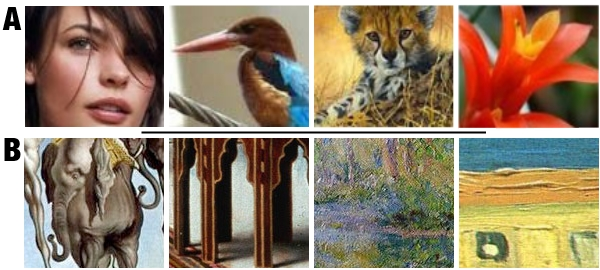
\includegraphics[width=1\linewidth]{stim.jpg}
\captionof{figure}{\color{DarkSlateGrey} Sample stimuli used at test, representing \textbf{A.} ecological concepts, \textbf{B.} artifical concepts.}
\end{center}\vspace{0.5cm}
%

%
%\section*{Experiment 1}
%
%Perceptual concept learning has been most often tested with ecologically valent stimuli (Shrier et al. 1984; Vonk \& MacDonald 2002; Marsh \& MacDonald 2008). We chose four commonly used classes of ecological stimuli (Shrier et al. 1987; Bhatt et al. 1988; Roberts \& Mazmanian 1988) (Figure 1A)  and trained three macaques to recognize all four concepts simultaneously, in a prespecified order.
%
%
%
%%------------------------------------------------
%
%\subsection*{Materials and Methods}
%
\textit{Subjects.} 7 male Rhesus macaques - 3 learned ecological concepts, 4 learned artificial (Figure 1).
%\textit{Apparatus}. Subjects performed tasks in operant chambers made of Plexiglas and stainless steel (53 cm x 48cm x 53 cm), enclosed within sound-attenuated booths (127 cm high x 97 cm wide x 97 cm deep). Each booth contained a pellet dispenser (Med Associates) that delivered a single 190-mg banana pellet (Bioserv) after every correct trial, as well as a closed-circuit camera. Subjects made responses by touching stimuli that were presented on a touch-sensitive 15 inch (38 cm) computer monitor in the chamber. All experimental tasks were programmed using Real Studio (formerly RealBASIC) and controlled by an iMac computer (model: MA710xx/A). Unless otherwise noted, the apparatus was identical to that employed by Subiaul and colleagues (2004).

\textit{Procedure}. Subjects were trained and tested using variations of the Simultaneous Chaining (SimChain) paradigm. Training was accomplished by presenting subjects with sequences in which the exemplars, drawn with replacement from very large stimulus banks, changed trial by trial. After learning the correct order of the concepts, performance was tested with 20 SimChains in which the stimuli were novel and did not change over the course of each session.







%%----------------------------------------------------------------------------------------
%%	EXPERIMENT 2
%%----------------------------------------------------------------------------------------
%
%\section*{Experiment 2}
%
%Having assessed macaques’ ability to simultaneously recognize distinct ecologically valid concepts, we turned to the ecological concept's oft-studied counterpart. Artificial concepts are usually examined in juxtaposition to ecological concepts; artificial and ecological foreground objects are paired with complementary or clashing artificial and ecological backgrounds, which has revealed that context is crucial: complementary backgrounds make recognition of foreground objects easier (Fize et al. 2011).
%
%Artificial classes of objects have previously included means of transport, furniture, utensils, tools, toys, and other objects that are distinctly man-made, predominantly immobile, and rigid (Fize et al. 2011, Sigala 2009). In our attempt to study artificial stimuli, we created classes of stimuli from the large bodies of work of prolific painters. Small samples were cropped from high-resolution images of paintings, such that the larger scope of each painting was not visible, leaving only local features, such as the texture and brushwork, to identify the artist (Figure 1B). These classes represent concepts that are man-made, but that are not directly analogous to objects or organisms found in the wild. Employing these stimulus sets, we trained and tested four new monkeys using the same paradigm as in Experiment 1.
%
%
%%------------------------------------------------
%
%\subsection*{Materials and Methods}
%
%\textit{Subjects.} Data were collected from 3 male rhesus monkeys (Macaca mulatta), Augustus, Coltrane, and Lashley. All subjects had extensive experience with the standard simultaneous chain task prior to the beginning of the experiment. Subjects were housed at the New York State Psychiatric Institute throughout the study. In addition to pellets obtained from performing tasks, subjects were given a mixed diet of primate chow and fruit immediately following daily testing. Water was available ad libitum.
%
%\textit{Apparatus}. Subjects performed tasks in operant chambers made of Plexiglas and stainless steel (53 cm x 48cm x 53 cm), enclosed within sound-attenuated booths (127 cm high x 97 cm wide x 97 cm deep). Each booth contained a pellet dispenser (Med Associates) that delivered a single 190-mg banana pellet (Bioserv) after every correct trial, as well as a closed-circuit camera. Subjects made responses by touching stimuli that were presented on a touch-sensitive 15 inch (38 cm) computer monitor in the chamber. All experimental tasks were programmed using Real Studio (formerly RealBASIC) and controlled by an iMac computer (model: MA710xx/A). Unless otherwise noted, the apparatus was identical to that employed by Subiaul and colleagues (2004).
%
%\textit{Procedure}. Subjects performed two closely related tasks . One was the simultaneous chaining task (Terrace 1984; 2005), hereafter identified as the “SimChain” task. In this task, a set of visual stimuli are presented on-screen simultaneously. These stimuli collectively are referred to as a “list,” because rewards are only earned if they are touched in the correct order. Subjects making a series of touches either receive a reward when every list item is touched in order, or they receive a time-out lasting 6 seconds upon the first touch to an item out of order. The particulars of the SimChain task were identical to those described by Jensen and colleagues (2013).
%The second task, which is novel to this study, is the Concept Chaining task. As in the SimChain task, a Concept Chain consists of a set of stimuli, simultaneously presented, that must be touched in the correct order to receive a reward. However, unlike a SimChain (in which the list items are fixed throughout a session), the stimuli in a Concept Chain are drawn randomly from related sets on every trial. For example, if the first item in the Concept Chain is “flowers,” then the first list item presented on every trial will be a different randomly selected picture of a flower, drawn from an image bank. This includes scenarios in which trial-unique stimuli are employed, in which the images used on a single trial have never been seen before by subjects, and are never seen again on any subsequent trial.
%
%The culmination of training was to perform the Concept Chain task with all stimuli changing on every trial. 
%Once all data using the Concept Chain had been collected, subjects then completed 20 sessions using the traditional SimChain task. Each session presented them with a fixed list of four never-before-seen stimuli belonging to the previously learned ordered classifications. Performance on these “fixed conceptual lists” was compared to SimChain performance during sessions that used arbitrary stimuli unrelated to the trained classifications.
%
%\subsection*{Results and Discussion}



%----------------------------------------------------------------------------------------
%	RESULTS 
%----------------------------------------------------------------------------------------

\section*{Results}

At the end of ecological concept training, subjects were highly proficient at selecting never-before-seen trial-unique stimuli in an order prescribed by their categories, successfully earning a reward on 51.3\% (Augustus), 58.8\% (Coltrane), and 53.2\% (Lashley) of trials. Chance performance on a 4-item SimChain gives a 4.16\% reward rate.\vspace{0.1cm}

At test, reward rates were significantly higher for concept ordered lists, than for lists composed of arbitrary stimuli:
{\small
\begin{description}
\item[] Augustus - 13.7\% arbitrary vs. 65.0\% categorical ($\chi^2=$636, df=1, p\textless 0.001).
\item[] Coltrane - 71.6\% arbitrary vs. 86.0\% categorical ($\chi^2=$63.1, df=1, p\textless 0.001). 
\item[] Lashley - 34.9\% arbitrary vs. 65.4\% categorical ($\chi^2=$148, df=1, p\textless 0.001).
\end{description}
}

Additionally, performance in both tasks was characterized using a learning curve function \cite{thurstone1919}. Model parameters significantly differed (p\textless 0.001) between categorical and arbitrary performance curves (Figure 2).

\begin{center}\vspace{1cm}
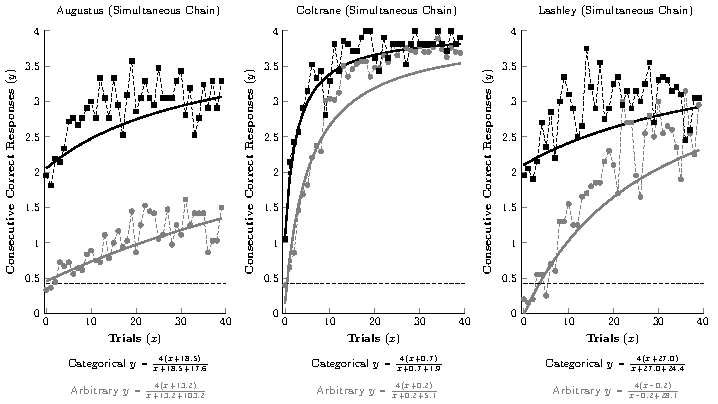
\includegraphics[width=0.8\linewidth]{Figure-02.pdf}
\captionof{figure}{\color{DarkSlateGrey} Learning curves of three macaques tested on 20 trials of a simultaneous chain using trial unique ecological concept stimuli. }
\end{center}\vspace{1cm}

The painting stimuli were considerably more difficult to train. Reward rates were similar across subjects: 28.3\% (Benedict), 27.5\% (Horatio), 33.5\% (MacDuff), and 33.0\% (Prospero), by the end of training.\vspace{0.1cm}

Trial reward rates:
{\small
\begin{description}
\item[] Benedict - 33.7\% arbitrary vs. 50.2\% categorical ($\chi^2=$74.2, df=1, p\textless 0.001)
\item[] Horatio - 41.2\% arbitrary vs. 44.4\% categorical ($\chi^2=$2.59, df=1, p = 0.11)
\item[] MacDuff - 40.7\% arbitrary vs. 31.7\% categorical ($\chi^2=$16.14, df=1, p\textless 0.001)
\item[] Prospero - 43.3\% arbitrary vs. 35.5\% categorical ($\chi^2=$15.50, df=1, p\textless 0.001)
\end{description}
}

Comparable models were generated (Figure 3). Three of four subjects showed significant differences in model parameters (p\textless 0.001), but one subject did not (Prospero).
	

\begin{center}\vspace{1cm}
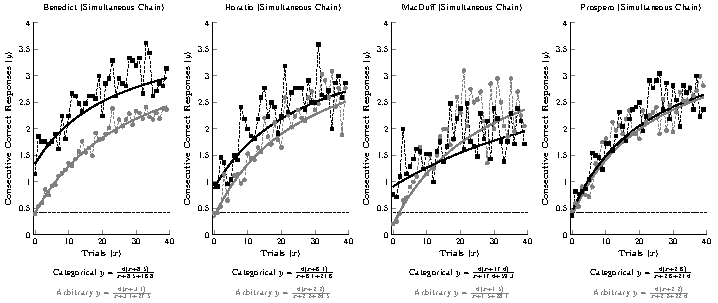
\includegraphics[width=1\linewidth]{Figure-04.pdf}
\captionof{figure}{\color{DarkSlateGrey} Learning curves of four macaques tested on 20 trials of a simultaneous chain using trial unique painting stimuli.}
\end{center}\vspace{1cm}
%
%\begin{wraptable}{l}{12cm} % Left or right alignment is specified in the first bracket, the width of the table is in the second
%\begin{tabular}{l l l}
%\toprule
%\textbf{Treatments} & \textbf{Response 1} & \textbf{Response 2}\\
%\midrule
%Treatment 1 & 0.0003262 & 0.562 \\
%Treatment 2 & 0.0015681 & 0.910 \\
%Treatment 3 & 0.0009271 & 0.296 \\
%\bottomrule
%\end{tabular}
%\captionof{table}{\color{Green} Table caption}
%\end{wraptable}
%


%----------------------------------------------------------------------------------------
%	CONCLUSIONS
%----------------------------------------------------------------------------------------

\color{Maroon} % SaddleBrown color for the conclusions to make them stand out
\color{Black}


\section*{Summary}

\begin{itemize}
\item With ecological stimuli, macaques were proficient at classifying a large training set and novel exemplars.
\item With artificial stimuli, macaques were able to classify a large training set.
\item 3 out of 4 subjects displayed conceptual knowledge during transfer.
\item Macaques appear able to classify stimuli based on gestalt properties, reflecting a generalizable ability to form abstract perceptual concepts.
\end{itemize}

\color{Black} % Set the color back to DarkSlateGray for the rest of the content

%----------------------------------------------------------------------------------------
%	FUTURE
%----------------------------------------------------------------------------------------

\color{Maroon}
\section*{Where to go from here}

\begin{itemize}
\item Compare concept chaining performance to baseline SimChain performance and personality measures.
\item Replicate in other species, notably humans, chimps.
\item Explore the objective difficulty and attributes of painting stimuli.
\end{itemize}	

 %----------------------------------------------------------------------------------------
%	REFERENCES
%----------------------------------------------------------------------------------------

\color{Black}
{\footnotesize
\nocite{*} % Print all references regardless of whether they were cited in the poster or not
\bibliographystyle{apacite} % Plain referencing style
\bibliography{apabibl} % Use the example bibliography file sample.bib
}

%%----------------------------------------------------------------------------------------
%%	ACKNOWLEDGEMENTS
%%----------------------------------------------------------------------------------------
%
%\section*{Acknowledgements}
%
%Etiam fermentum, arcu ut gravida fringilla, dolor arcu laoreet justo, ut imperdiet urna arcu a arcu. Donec nec ante a dui tempus consectetur. Cras nisi turpis, dapibus sit amet mattis sed, laoreet.
%
%%----------------------------------------------------------------------------------------

\end{multicols}
\end{document}